\section{Transaktionen}
SQL: BEGIN, COMMIT, ROLLBACK;

Transaktionsabbrüche durch integritätsverletzungen, Konsistenzbedinungen, Speicher voll, Verbindungsabbruch, Systemausfall ...

\subsection{Anomalien}
\begin{enumerate}
\item Lost-Update: Überschriebene Änderungen
\item Dirty-Read: Lesen eines nicht committeten Wertes
\item Unrepeatable Read: durch commit anderer Transaktion liefert die selbe anfrage nicht das gleiche Ergebnis
\item Phantom Read: Einfügen von Datensätzen durch andere Transaktion
\end{enumerate}

Serialisierbar: Gleiches Ergebnis wie bei hintereinanderausführung der Transaktion
$\Leftrightarrow$ kein Zyklus im Abhängigkeitsgraph

z.B. $R_1(a), W_2(a), R_3(a), W_1(a)$
\tikzset{ LabelStyle/.style = { rectangle, rounded corners, draw, minimum width = 2em, font =fseries }, VertexStyle/.append style = { inner sep=5pt, font = \Large\bfseries}, EdgeStyle/.append style = {->,bend left =20}}
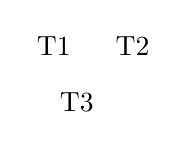
\begin{tikzpicture}
\tikzset{EdgeStyle/.append style = {->,bend left =20,black}}
\node(1){T1}; \node(2)[right of=1]{T2}; \node(3)[below left of=2]{T3};
\Edge(1)(2){a}; \Edge(2)(3){a}; \Edge (3)(1){a}; \Edge(2)(1){a};
\end{tikzpicture}
 => nicht serialisierbar

Sperren: Shared-Locks (s) beim Lesen, Exklusiv-Locks (X) beim Schreiben

\subsection{Zwei-Phasen-Protokoll:} Sperren werden erst am Transaktionsende (vor commit) wieder freigegeben

\begin{tabular}{|c|c|}
\hline
T1 & T2 \\
\hline
Slock(a), read(a); & \\
& Slock(a), read(a);\\
Wait(Xlock(a)) & \\
& Wait(Xlock(a))\\
& DEADLOCK => Rollback;\\
write(a)&\\
unlock(a);&\\
commit;&\\
\hline
\end{tabular}




SQL-Isolationssteuerung: SET TRANSACTION ISOLATION LEVEL \{ READ UNCOMMITTED | READ COMMITTED | REPEATABLE READ | SERIALIZABLE \}

Multi-Version-Concurrency-Control: Snapshots: keine Lesesperren, änderungen erzeugen kopie

\section{Fehlerbehandlung}
Lokaler Fehler in Transaktion: Rollback der Transaktion\\

Verlust des Hauptspeichers:Durch Logging der Aktionen, nach Crash Undo nicht abgeschlossener Aktionen, Redo abgeschlossener.\\
Verlust des externen Speichers: Backup einspielen, inkrementell log-einspielen\\


Write-Ahead-Logging: festhalten aller änderungen vor commit, bei rollback wiederherstellung aus transaktionslog;\\
Log beinhaltet Undo- und Redo-Informationen; (vor und nach zustand)\\
logisches Logging: protokollierung der Befehle\\
physisches Logging: Zustandkopien\\

Steal-noforce:
Steal: gepufferte seiten können von anderer Transaktion eingelagert werden, zusammen mit zugehörigem Undo-logeintrag\\
NoForce: committete Seiten müssen nicht sofort auf platte geschrieben, aber im Redo-log vermerkt werden.

Ablauf: Redo-lauf (durchführen der geloggten änderungen); Undo-lauf: rollback nicht committeter änderungen

Recovery time objective: max. ausfallzeit; recovery point objective: max. Datenverlust

\section{Dateiorganisation}
Heap-Dateiorganisation: Speichern von Datensätzen in Einfügereihenfolge => unsortiert
Einfügen am ende, löschen suchen und setzen eines Löschbits, suchen: sequenziell oder index;

sequentielle-Dateiorganisation: sortierte speicherung;
einfügen: suchen, anhängen und dann sortieren der Seite; löschen: suchen und löschbit setzen; suchen über index

Index: B-Baum-Struktur; clustered Index: Segmente selbst sind sortiert;  
CREATE INDEX <name> ON 	<tabelle>(<spalte(n)>); DROP INDEX <name>

\section{Anfrageverarbeitung}

SQL -> Query Execution Plan:\\
Parsen der Anfrage -> Operatorengraph; // hierbei Standardisieren und vereinfachen  \\
\textbf{KNF} : (a and b) or (c and d); \\
\rule{2em}{0em}deMorgan: $\overline{a AND b} = \overline{a} OR \overline{b}$\\
\rule{2em}{0em}\textcolor{white}{deMorgan :} $\overline{a OR b} = \overline{a} AND \overline{b}$\\

\definecolor{darkgreen}{rgb}{0.2,0.8,0.2}
\newcommand{\proj}{\textcolor{red}{\ensuremath{\pi_{k.nr,p.nr}}}}
\newcommand{\joink}{\textcolor{darkgreen}{\ensuremath{\bowtie_{k.knr = a.knr}}}}
\newcommand{\joina}{\textcolor{darkgreen}{\ensuremath{\bowtie_{a.anr = p.anr}}}}
\newcommand{\selk}{\textcolor{blue}{\ensuremath{\sigma_{k.name = 'x'}} }}
\newcommand{\selor}{\textcolor{blue}{\ensuremath{\sigma_{a.anr > 10 OR k.knr >10 }}}}
\newcommand{\grpi}[1]{\textcolor{gray}{ \ensuremath{\pi_{ #1 }} }}

\begin{minipage}{0.25\textwidth}
SELECT $\underbrace{k.name, p.nr}_{ \proj }$ \\
FROM Knd k JOIN Auftr a $\underbrace{ ON k.knr = a.knr}_{\joink}$ \\
JOIN Auftrpos p $\underbrace{ ON a.anr =p.anr}_{\joina} $\\
WHERE $\underbrace{k.name = 'x'}_{\selk}$ AND\\
$\underbrace{(a.anr > 10 OR k.knr >10)}_{\selor}$
\end{minipage}
% $\Leftrightarrow$
% 
%\begin{tikzpicture}[level distance=3em,sibling distance=7em]
%\node{\proj} 
%child{ node{\selk}
%child{ node{\selor}
%child{ node{\joina}
%child{ node{\joink}
%child{ node{Knd k}}
%child{ node{Auftr a}}
%}
%child{ node{Auftrp p}
%}}}}
%;
%\end{tikzpicture}
%$\Leftrightarrow$
\begin{minipage}{0.25\textwidth}
\begin{tikzpicture}[level distance=3em,sibling distance=5.5em ,level 2/.style={sibling distance=7em} ]
\node{\proj} 
child{ node{\joina}
child{ node{\grpi{a.nr,k.nr}}
child{ node{\selor}
child{ node{\joink}
child{ node{\grpi{k.nr}}
child{ node{\selk}
child{ node{Knd k}}}}
child{ node{\grpi{a.knr,a.anr}}
child{ node{Auftr a}}}
}}}
child{ node{\grpi{p.anr}}
child{ node{Auftrpos p}
}}}
;
\end{tikzpicture}
\end{minipage}

\textbf{\textcolor{red}{HINWEIS:}} konstruiere von unten nach oben.

\subsection{Kostenschätzung}
Anhand von Statistiken, Histogrammen, etc.; evtl. Hints für Optimizer

\textbf{Kardinalität}: |a|: Anzahl der gelieferten Datensätze \\
\textbf{Selektivität}: Sel(a): \% der Datensätze im vergleich zu gesamtzahl;\\
NumBlocks: $\dfrac{|R|\cdot Laenge_{Datensatz}}{Blocksize}$

Levels(I(R,A)): Höhe des Index auf A

Sel(P) = $\dfrac{\text{zurückgegebene DS}}{gesamt DS}$

Attribut = 'sth' => Sel(A) = 1/|A|

Attribut IN $\{c_1,c_2, \dots , c_n\}$ => Sel(A) = n / |A|

A >c => Sel(A) = $\dfrac{A_{max} -c }{A_{max} - A_{min}}$

$P_1 AND P_2$ => $Sel(P_1) \cdot Sel(P_2)$

$P_1 OR P_2$ => $Sel(P_1) + Sel(P_2) + Sel(P_1 AND P_2$

\section{Plan-Operatoren}
\begin{itemize}
\item Full-Table-Scan: durchsuche gesamte Tabelle: Cost = NumBlocks(R)
\item Index-Scan: Suche anhand index: Cost = Levels(Index) + Sel(P) $\cdot$|R|
\item Nested-Loop-Join: für jeden Block: durchlaufe die andere Tabelle\\
Ohne Index: Cost= NumBlocks(R) * NumBlocks(S) ; \\
mit Index Cost= NumBlocks(R) * Cost(IndexScan)
\item Merge-Join: Sortiere die Relationen nach Join-Attribut; paralleles Durchlaufen der Paare in den sortierten Relationen;\\
Cost: Cost(Sort(R)) +Cost(Sort(S)) + NumBlocks(S) + NumBlocks(R)
\item Hash-Join: Teile kleinere Relation K in h Abschnitte, wird im RAM gehalten;\\
durchlaufe die Abschnitte: Erstelle Hashtabelle, prüfe für jeden Datensatz der 2. Relation JOIN-Bedingung mit den Zugehörigen Werten; Cost: NumBlocks(R) + x * NumBlocks(S)

\end{itemize}